\documentclass[article]{jss}
\usepackage{longtable}
%%%%%%%%%%%%%%%%%%%%%%%%%%%%%%
%% declarations for jss.cls %%%%%%%%%%%%%%%%%%%%%%%%%%%%%%%%%%%%%%%%%%
%%%%%%%%%%%%%%%%%%%%%%%%%%%%%%

%% almost as usual
\author{Douglas Bates\\University\ of Wisconsin-Madison \And 
        Colin Longhurst \\University of Wisconsin-Madison}
\title{Comparing Optimization Algorithms in the Fitting of Linear Mixed Models: Evaluating Speed and Accuracy using \pkg{lme4} in R and \pkg{lmm} in Julia}

%% for pretty printing and a nice hypersummary also set:
\Plainauthor{Douglas Bates, Colin Longhurst} %% comma-separated
\Plaintitle{Comparing Optimization Algorithms in the Fitting of Linear Mixed Models: Evaluating Speed and Accuracy using lme4 in R and lmm in Julia} %% without formatting
\Shorttitle{\pkg{Timings}: A Package for the Evaluation of Optimization Algorithms} %% a short title (if necessary)

%% an abstract and keywords
\Abstract{
The \pkg{Timings} package allows for the comparison of several optimizers, in both \proglang{R} and \proglang{Julia}, used in the fitting of various linear mixed models. In \proglang{R} the optimizers are called by lmer from the \pkg{lme4} package (version 1.1-8). In \proglang{Julia} the optimizers are called by lmm from \pkg{MixedModels} package.  From the \pkg{Timings} package, conclusions regarding an optimizers relative speed, accuracy and general effectiveness of different optimizers paired with different types of models (ranging from simple to complex) can easily be drawn and interpretted.  \\
  There are differences in the model formulations in \pkg{lme4} and in \pkg{MixedModels}. The numerical representation of the model in \pkg{lme4} and the method of evaluating the optimizers, described in this paper, is the same for all models. In \pkg{MixedModels} there are specialized representations for some model forms, such as models with a single grouping factor for the random effects. Some of the specialized representations allow for evaluation of the gradient of the objects, which can enhance convergence (but, interestingly, sometimes can impede convergence).
}
\Keywords{optimizers, mixed models, linear mixed models, lme4, lmm, \proglang{R}, \proglang{Julia}}
\Plainkeywords{optimizers, mixed models, linear mixed models, lme4, lmm} %% without formatting
%% at least one keyword must be supplied

%% publication information
%% NOTE: Typically, this can be left commented and will be filled out by the technical editor
%% \Volume{50}
%% \Issue{9}
%% \Month{June}
%% \Year{2012}
%% \Submitdate{2012-06-04}
%% \Acceptdate{2012-06-04}

%% The address of (at least) one author should be given
%% in the following format:
\Address{
  Douglas Bates\\
  Emeritus Professor\\
  Department of Statistics\\
  University of Wisconsin-Madison\\
  1300 University Ave
  Madison, WI 53706-1685
  U.S.A.\\
  E-mail: \email{dmbates@stat.wisc.edu}\\
  Github URL: \url{https://github.com/dmbates}
}
%% It is also possible to add a telephone and fax number
%% before the e-mail in the following format:
%% Telephone: +43/512/507-7103
%% Fax: +43/512/507-2851

%% for those who use Sweave please include the following line (with % symbols):
%% need no \usepackage{Sweave.sty}

%% end of declarations %%%%%%%%%%%%%%%%%%%%%%%%%%%%%%%%%%%%%%%%%%%%%%%


\begin{document}



%% include your article here, just as usual
%% Note that you should use the \pkg{}, \proglang{} and \code{} commands.

\section[Introduction]{Introduction}
%% Note: If there is markup in \(sub)section, then it has to be escape as above.



Mauris ac lectus sagittis, mollis diam porttitor, efficitur purus. Duis ut eros vitae dolor vulputate sagittis. Aenean viverra, dui in interdum consectetur, lectus elit placerat urna, dictum ultricies ex justo eget est. In at leo quam. Suspendisse eros nulla, gravida nec suscipit vel, egestas eget neque. Etiam pharetra, nisl nec viverra ultricies, mauris lectus facilisis velit, vel aliquam ipsum lorem ut sem. Nulla ornare, justo at tempus blandit, nulla urna porta ligula, id dictum mi est ac massa. Quisque at lacus neque. Pellentesque est nulla, dignissim eget lobortis ut, vehicula at erat. Aenean ornare lacus mattis, elementum elit vel, tempor risus. In in purus tempor lacus imperdiet rhoncus nec nec tortor. Duis sagittis nisl ante, id egestas neque tristique fermentum. Fusce aliquet, odio non auctor aliquet, purus orci venenatis purus, sit amet pulvinar nisi est at dolor. Pellentesque lobortis dui eros, et ultricies tellus ultrices at. Ut sit amet interdum justo. Integer placerat vehicula interdum. 


\section[Methods]{Methods}


To provide consistency we have copied all the data sets used in the
timings to the \pkg{Timings} package itself. We have done all timings
on the same computer. This computer has a relatively recent Intel
processor and we used the
\href{https://software.intel.com/en-us/intel-mkl}{Intel Math Kernel
Library (MKL)} with \proglang{Julia}. We attempted to use
\href{www.revolutionanalytics.com/revolution-r-open}{Revolution R Open
(RRO)} as the \proglang{R} implementation as it can be configured with \pkg{MKL}.
However, we ran into version problems with this so we used the standard
Ubuntu version of \proglang{R} linked against OpenBLAS, which is also
multi-threaded.

Variables were renamed in the pattern: 

\begin{itemize}
\item \textbf{Y} the response 
\item \textbf{A}, \textbf{B}, \dots{} categorical covariates 
\item \textbf{G},\textbf{H}, \textbf{I}, \dots{} grouping factors for random effects 
\item \textbf{U}, \textbf{V}, \dots{} (skipping \textbf{Y}) continuous covariates
\end{itemize}


The timing results are saved in \href{http://json.org}{JSON (JavaScript
Object Notation)} files in the directory accessible as

\begin{Schunk}
\begin{Sinput}
> system.file("JSON",package="Timings")
\end{Sinput}
\end{Schunk}

within \pkg{R}. The directory name will end with
\texttt{./Timings/inst/JSON/} in the package source directory, for
example the result of cloning the
\href{https://github.com/Stat990-033/Timings}{github repository}. There
is one \texttt{.json} file for each data set. Each such file contains
results on timings of one or more models.

The \pkg{Timings} package for \proglang{R} provides a \texttt{retime}
function that takes the name of one of these JSON files and, optionally,
the name of a file with the updated timings. Similarly there are some
source files for \pkg{Julia} retimings.

\begin{Schunk}
\begin{Sinput}
> include("../julia/retime.jl")
> retime("../JSON/Alfalfa.json","/tmp/Alfalfa.json")
> retime("../JSON/Alfalfa.json","/tmp/Alfalfa.json")
\end{Sinput}
\end{Schunk}


  The timing was repeated so that compilation time is not included in the
results. This repetition is only needed once per session.

A careful examination of these results shows that the main differences
in the \pkg{Julia} timings (the \pkg{R} timings are merely reported, not evaluated)
are that the \texttt{LN\_BOBYQA} and \texttt{LD\_MMA} optimizers are
much faster in the second run. This is because much of the code needs to
be compiled the first time that a derivative-free optimizer and a
derivative-based optimizer are used.

The names of the optimizers used with \texttt{lmm} are those from the
\pkg{NLopt} package for \proglang{Julia}. Names that begin with \texttt{LD\_} are gradient-based
methods. Names that begin with \texttt{LN\_} are derivative-free
methods. There is one other derivative-free method, \texttt{LN\_PRAXIS},
available in the \pkg{NLopt} package but, for some reason, it can
hang on very simple problems like this. Frequently we omit it.

The optimizers used with \texttt{lmer} include the \texttt{Nelder\_Mead}
optimizer built into the \pkg{lme4} package, the \texttt{bobyqa}
optimizer from the
\pkg{minqa} package, the derivative-free optimizers from the
\pkg{nloptr} package and several optimizers from the
\pkg{optimx} pacakge.

The \texttt{optimx:bobyqa} optimizer is just a wrapper around
\texttt{bobyqa} (bounded optimization by quadratic approximation) from
the \pkg{minqa} package and should provide results similar to those
from the \texttt{bobyqa} optimizer. For some reason the number of
function evaluations is not reported for the version in \pkg{optimx}.

The optimizers from \pkg{nloptr} (i.e.~those whose names begin with
\texttt{NLOPT\_LN\_}) use the same underlying code as do the similarly
named optimizers in the \pkg{NLopt} package for \proglang{Julia}. The
number of iterations to convergence should be similar for the same
underlying code, although not nessarily exactly the same because the
evaluation of the objective in \proglang{R} and in \proglang{Julia} may
produce slightly different answers. Also the convergence criteria in the
\proglang{Julia} version are more strict than those in the \proglang{R}
version

Also shown are the value of the criterion (negative twice the
log-likelihood, lower is better) achieved, the elapsed time and the
number of function and gradient evaluations. The \texttt{nopt} value is
the number of parameters in the optimization problem. \texttt{mtype} is
the model type in the \proglang{Julia} code. There are special methods for
solving the penalized least squares (PLS) problem, and for evaluating
the objective and its gradient when there is only one grouping factor
for the random effects. The model type is called \texttt{PLSOne}.

The \texttt{Alfalfa} example is a particularly easy one and all of the
optimizerws converge to an objective value close to -10.81023 in less
than 0.6 seconds.

\section[Results]{Results}

For the \texttt{Alfalfa} data there is not much of a burden in refitting
the model with all the \textbf{Julia} optimizers just to get the table
shown above. But other examples can take an hour or more to converge and
we don't really need to refit them every time. The \texttt{tabulate.jl}
file contains a function \texttt{optdir} to create a \texttt{DataFrame}
from the results of all the model fits.

\begin{Schunk}
\begin{Sinput}
> include("../julia/tabulate.jl")
> res = optdir("../JSON");
\end{Sinput}
\end{Schunk}


\begin
{center}
% latex table generated in R 3.1.3 by xtable 1.7-4 package
% Thu Sep 24 15:26:30 2015
\begin{table}[!htp]
\centering
\begin{tabular}{rllrrrrrr}
  \hline
 & opt & dsname & n & p & np & excess & time & reltime \\ 
  \hline
1 & LD\_CCSAQ & Alfalfa &  72 &  12 &   1 & 0.00 & 0.00 & 1.13 \\ 
  2 & LD\_CCSAQ & AvgDailyGain &  32 &   8 &   1 & 0.00 & 0.00 & 0.82 \\ 
  3 & LD\_CCSAQ & AvgDailyGain &  32 &   5 &   1 & 0.00 & 0.00 & 0.93 \\ 
  4 & LD\_CCSAQ & BIB &  24 &   8 &   1 & 0.00 & 0.00 & 0.79 \\ 
  5 & LD\_CCSAQ & Bond &  21 &   3 &   1 & 0.00 & 0.00 & 1.03 \\ 
  6 & LD\_CCSAQ & bs10 & 1104 &   4 &  20 & 0.00 & 1.10 & 4.44 \\ 
  7 & LD\_CCSAQ & bs10 & 1104 &   4 &   8 & 39.99 & 0.04 & 0.56 \\ 
  8 & LD\_CCSAQ & cake & 270 &  18 &   1 & 0.00 & 0.00 & 1.37 \\ 
  9 & LD\_CCSAQ & Cultivation &  24 &   6 &   1 & 0.00 & 0.00 & 0.99 \\ 
  10 & LD\_CCSAQ & Demand &  77 &   5 &   2 & 3.22 & 0.01 & 0.81 \\ 
  11 & LD\_CCSAQ & dialectNL & 225866 &   4 &   6 & 0.00 & 6.99 & 3.99 \\ 
  12 & LD\_CCSAQ & Dyestuff2 &  30 &   1 &   1 & 0.00 & 0.00 & 0.68 \\ 
  13 & LD\_CCSAQ & Dyestuff &  30 &   1 &   1 & 0.00 & 0.00 & 1.02 \\ 
  14 & LD\_CCSAQ & ergoStool &  36 &   4 &   1 & 0.00 & 0.00 & 1.10 \\ 
  15 & LD\_CCSAQ & Exam & 4059 &   5 &   1 & 0.00 & 0.01 & 1.19 \\ 
  16 & LD\_CCSAQ & Exam & 4059 &   6 &   1 & 0.00 & 0.01 & 1.32 \\ 
  17 & LD\_CCSAQ & Gasoline &  32 &   2 &   1 & 0.00 & 0.00 & 0.82 \\ 
  18 & LD\_CCSAQ & gb12 & 512 &   8 &  20 & 0.00 & 3.52 & 17.48 \\ 
  19 & LD\_CCSAQ & gb12 & 512 &   8 &   8 & 103.18 & 0.02 & 0.56 \\ 
  20 & LD\_CCSAQ & HR & 120 &   7 &   3 & 0.00 & 0.01 & 1.22 \\ 
  21 & LD\_CCSAQ & Hsb82 & 7185 &   5 &   1 & 192.73 & 0.01 & 0.49 \\ 
  22 & LD\_CCSAQ & IncBlk &  24 &   8 &   1 & 0.56 & 0.00 & 0.66 \\ 
  23 & LD\_CCSAQ & kb07 & 1790 &   8 &  72 & 8.21 & 17.47 & 4.12 \\ 
  24 & LD\_CCSAQ & Mississippi &  37 &   3 &   1 & 0.93 & 0.00 & 0.67 \\ 
  25 & LD\_CCSAQ & mm0 & 69588 &   4 &   6 & 0.00 & 4.83 & 4.40 \\ 
  26 & LD\_CCSAQ & Oxboys & 234 &   2 &   3 & 136.79 & 0.02 & 0.71 \\ 
  27 & LD\_CCSAQ & PBIB &  60 &  15 &   1 & 0.00 & 0.00 & 1.00 \\ 
  28 & LD\_CCSAQ & Penicillin & 144 &   1 &   2 & 0.00 & 0.01 & 4.94 \\ 
  29 & LD\_CCSAQ & Semiconductor &  48 &  16 &   1 & 0.00 & 0.00 & 1.05 \\ 
  30 & LD\_CCSAQ & SIMS & 3691 &   2 &   3 & 3.61 & 0.13 & 0.99 \\ 
  31 & LD\_CCSAQ & sleepstudy & 180 &   2 &   3 & 0.00 & 0.01 & 1.75 \\ 
  32 & LD\_CCSAQ & sleepstudy & 180 &   2 &   2 & 0.00 & 0.00 & 1.13 \\ 
  33 & LD\_CCSAQ & TeachingII &  96 &  12 &   1 & 0.00 & 0.00 & 0.93 \\ 
  34 & LD\_CCSAQ & Weights & 399 &   6 &   3 & 99.13 & 0.02 & 0.51 \\ 
  35 & LD\_CCSAQ & WWheat &  60 &   2 &   3 & 18.20 & 0.01 & 0.68 \\ 
   \hline
\end{tabular}
\end{table}\end {center}


The \texttt{time} column is the time in seconds to converge. The
\texttt{reltime} column is the time relative to the \texttt{LN\_BOBYQA}
optimizer in the \pkg{MixedModels} package for \proglang{Julia}.

For \proglang{Julia} the time column is the time in seconds to converge. The reltime column is the time relative to the LN_BOBYQA optimizer in the \pkg{MixedModels} package for \proglang{Julia}.

\begin
{center}
% latex table generated in R 3.1.3 by xtable 1.7-4 package
% Thu Sep 24 15:26:30 2015
\begin{tabular}{rllrrrrrr}
  \hline
 & opt & dsname & n & p & np & excess & time & reltime \\ 
  \hline
560 & NLOPT\_LN\_BOBYQA & Alfalfa &  72 &  12 &   1 & 0.00 & 0.04 & 27.52 \\ 
  561 & NLOPT\_LN\_BOBYQA & Animal &  20 &   1 &   2 & 0.00 & 0.02 & 13.92 \\ 
  562 & NLOPT\_LN\_BOBYQA & Assay &  60 &  31 &   2 & 0.00 & 0.03 & 10.80 \\ 
  563 & NLOPT\_LN\_BOBYQA & AvgDailyGain &  32 &   8 &   1 & 0.00 & 0.02 & 11.70 \\ 
  564 & NLOPT\_LN\_BOBYQA & AvgDailyGain &  32 &   5 &   1 & 0.00 & 0.02 & 13.70 \\ 
  565 & NLOPT\_LN\_BOBYQA & BIB &  24 &   8 &   1 & 0.00 & 0.02 & 12.61 \\ 
  566 & NLOPT\_LN\_BOBYQA & Bond &  21 &   3 &   1 & 0.00 & 0.02 & 23.27 \\ 
  567 & NLOPT\_LN\_BOBYQA & bs10 & 1104 &   4 &  20 & 0.00 & 4.66 & 18.88 \\ 
  568 & NLOPT\_LN\_BOBYQA & bs10 & 1104 &   4 &   8 & 0.00 & 1.06 & 15.65 \\ 
  569 & NLOPT\_LN\_BOBYQA & cake & 270 &  18 &   1 & 0.00 & 0.05 & 22.08 \\ 
  570 & NLOPT\_LN\_BOBYQA & Chem97 & 31022 &   1 &   2 & 0.00 & 0.63 & 3.94 \\ 
  571 & NLOPT\_LN\_BOBYQA & Chem97 & 31022 &   2 &   2 & 0.00 & 0.56 & 3.60 \\ 
  572 & NLOPT\_LN\_BOBYQA & Cultivation &  24 &   6 &   1 & 0.00 & 0.02 & 23.10 \\ 
  573 & NLOPT\_LN\_BOBYQA & d3 & 130418 &   2 &   9 & 0.00 & 231.30 & 2.16 \\ 
  574 & NLOPT\_LN\_BOBYQA & Demand &  77 &   5 &   2 & 0.00 & 0.03 & 3.81 \\ 
  575 & NLOPT\_LN\_BOBYQA & dialectNL & 225866 &   4 &   6 & 0.00 & 16.88 & 9.64 \\ 
  576 & NLOPT\_LN\_BOBYQA & Dyestuff2 &  30 &   1 &   1 & 0.00 & 0.05 & 62.58 \\ 
  577 & NLOPT\_LN\_BOBYQA & Dyestuff &  30 &   1 &   1 & 0.00 & 0.02 & 24.87 \\ 
  578 & NLOPT\_LN\_BOBYQA & egsingle & 7230 &   5 &   2 & 0.00 & 0.17 & 2.39 \\ 
  579 & NLOPT\_LN\_BOBYQA & ergoStool &  36 &   4 &   1 & 0.00 & 0.02 & 17.25 \\ 
  580 & NLOPT\_LN\_BOBYQA & Exam & 4059 &   5 &   1 & 0.00 & 0.05 & 5.40 \\ 
  581 & NLOPT\_LN\_BOBYQA & Exam & 4059 &   6 &   1 & 0.00 & 0.05 & 6.33 \\ 
  582 & NLOPT\_LN\_BOBYQA & Gasoline &  32 &   2 &   1 & 0.00 & 0.02 & 14.30 \\ 
  583 & NLOPT\_LN\_BOBYQA & gb12 & 512 &   8 &  20 & 0.00 & 1.87 & 9.28 \\ 
  584 & NLOPT\_LN\_BOBYQA & gb12 & 512 &   8 &   8 & 0.00 & 0.42 & 10.77 \\ 
  585 & NLOPT\_LN\_BOBYQA & Genetics &  60 &   5 &   2 & 0.00 & 0.03 & 9.60 \\ 
  586 & NLOPT\_LN\_BOBYQA & HR & 120 &   7 &   3 & 0.00 & 0.02 & 3.29 \\ 
  587 & NLOPT\_LN\_BOBYQA & Hsb82 & 7185 &   5 &   1 & 0.00 & 0.07 & 3.52 \\ 
  588 & NLOPT\_LN\_BOBYQA & IncBlk &  24 &   8 &   1 & 0.00 & 0.02 & 12.89 \\ 
  589 & NLOPT\_LN\_BOBYQA & InstEval & 73421 &  28 &   2 & 0.00 & 10.06 & 4.28 \\ 
  590 & NLOPT\_LN\_BOBYQA & InstEval & 73421 &   2 &   3 & 0.00 & 15.82 & 3.63 \\ 
  591 & NLOPT\_LN\_BOBYQA & kb07 & 1790 &   8 &  72 & 0.01 & 311.03 & 73.43 \\ 
  592 & NLOPT\_LN\_BOBYQA & kb07 & 1790 &   8 &  16 & 0.00 & 18.50 & 26.31 \\ 
  593 & NLOPT\_LN\_BOBYQA & Mississippi &  37 &   3 &   1 & 0.00 & 0.02 & 21.53 \\ 
  594 & NLOPT\_LN\_BOBYQA & mm0 & 69588 &   4 &   6 & 0.00 & 26.20 & 23.88 \\ 
  595 & NLOPT\_LN\_BOBYQA & Oxboys & 234 &   2 &   3 & 0.00 & 0.03 & 1.35 \\ 
  596 & NLOPT\_LN\_BOBYQA & Pastes &  60 &   1 &   2 & 0.00 & 0.02 & 9.51 \\ 
  597 & NLOPT\_LN\_BOBYQA & PBIB &  60 &  15 &   1 & 0.00 & 0.02 & 13.14 \\ 
  598 & NLOPT\_LN\_BOBYQA & Penicillin & 144 &   1 &   2 & 0.00 & 0.02 & 8.65 \\ 
  599 & NLOPT\_LN\_BOBYQA & Poems & 275996 &   3 &   3 & 0.00 & 21.31 & 3.74 \\ 
  600 & NLOPT\_LN\_BOBYQA & ScotsSec & 3435 &   4 &   2 & 0.00 & 0.08 & 5.04 \\ 
  601 & NLOPT\_LN\_BOBYQA & Semi2 &  72 &   2 &   3 & 0.00 & 0.03 & 9.27 \\ 
  602 & NLOPT\_LN\_BOBYQA & Semiconductor &  48 &  16 &   1 & 0.00 & 0.02 & 15.96 \\ 
  603 & NLOPT\_LN\_BOBYQA & SIMS & 3691 &   2 &   3 & 0.00 & 0.15 & 1.10 \\ 
  604 & NLOPT\_LN\_BOBYQA & sleepstudy & 180 &   2 &   3 & 0.00 & 0.04 & 5.30 \\ 
  605 & NLOPT\_LN\_BOBYQA & sleepstudy & 180 &   2 &   2 & 0.00 & 0.02 & 8.62 \\ 
  606 & NLOPT\_LN\_BOBYQA & TeachingII &  96 &  12 &   1 & 0.00 & 0.02 & 15.38 \\ 
  607 & NLOPT\_LN\_BOBYQA & Weights & 399 &   6 &   3 & 0.00 & 0.04 & 1.13 \\ 
  608 & NLOPT\_LN\_BOBYQA & WWheat &  60 &   2 &   3 & 0.00 & 0.03 & 2.32 \\ 
   \hline
\end{tabular}\end {center}



\subsection[Convergence]{Proportion Converged}
The most important question regarding the optimizers is whether or not they have converged to the global optimum. We cannot test this directly. Instead we use a "crowd-sourced" criterion based on the minimum objective achieved by any of the algorithms. The difference between the objective achieved by a particular algorithm and this minimum is called the excess. In the summaries \texttt{excess} is rounded to 5 digits after the decimal so the minimum non-zero \texttt{excess} is $10^{-5}$.

\begin
{center}
% latex table generated in R 3.1.3 by xtable 1.7-4 package
% Thu Sep 24 15:26:30 2015
\begin{tabular}{rllr}
  \hline
 & opt & dsname & excess \\ 
  \hline
347 & LN\_BOBYQA & Alfalfa & 0.00 \\ 
  348 & LN\_BOBYQA & Animal & 0.00 \\ 
  349 & LN\_BOBYQA & Assay & 0.00 \\ 
  350 & LN\_BOBYQA & AvgDailyGain & 0.00 \\ 
  351 & LN\_BOBYQA & AvgDailyGain & 0.00 \\ 
  352 & LN\_BOBYQA & BIB & 0.00 \\ 
  353 & LN\_BOBYQA & Bond & 0.00 \\ 
  354 & LN\_BOBYQA & bs10 & 0.00 \\ 
  355 & LN\_BOBYQA & bs10 & 0.00 \\ 
  356 & LN\_BOBYQA & cake & 0.00 \\ 
  357 & LN\_BOBYQA & Chem97 & 0.00 \\ 
  358 & LN\_BOBYQA & Chem97 & 0.00 \\ 
  359 & LN\_BOBYQA & Cultivation & 0.00 \\ 
  360 & LN\_BOBYQA & d3 & 0.00 \\ 
  361 & LN\_BOBYQA & Demand & 0.00 \\ 
  362 & LN\_BOBYQA & dialectNL & 0.00 \\ 
  363 & LN\_BOBYQA & Dyestuff2 & 0.00 \\ 
  364 & LN\_BOBYQA & Dyestuff & 0.00 \\ 
  365 & LN\_BOBYQA & egsingle & 0.00 \\ 
  366 & LN\_BOBYQA & ergoStool & 0.00 \\ 
  367 & LN\_BOBYQA & Exam & 0.00 \\ 
  368 & LN\_BOBYQA & Exam & 0.00 \\ 
  369 & LN\_BOBYQA & Gasoline & 0.00 \\ 
  370 & LN\_BOBYQA & gb12 & 0.00 \\ 
  371 & LN\_BOBYQA & gb12 & 0.00 \\ 
  372 & LN\_BOBYQA & Genetics & 0.00 \\ 
  373 & LN\_BOBYQA & HR & 0.00 \\ 
  374 & LN\_BOBYQA & Hsb82 & 0.00 \\ 
  375 & LN\_BOBYQA & IncBlk & 0.00 \\ 
  376 & LN\_BOBYQA & InstEval & 0.00 \\ 
  377 & LN\_BOBYQA & InstEval & 0.00 \\ 
  378 & LN\_BOBYQA & kb07 & 0.02 \\ 
  379 & LN\_BOBYQA & kb07 & 0.00 \\ 
  380 & LN\_BOBYQA & Mississippi & 0.00 \\ 
  381 & LN\_BOBYQA & mm0 & 0.00 \\ 
  382 & LN\_BOBYQA & Oxboys & 0.00 \\ 
  383 & LN\_BOBYQA & Pastes & 0.00 \\ 
  384 & LN\_BOBYQA & PBIB & 0.00 \\ 
  385 & LN\_BOBYQA & Penicillin & 0.00 \\ 
  386 & LN\_BOBYQA & Poems & 0.00 \\ 
  387 & LN\_BOBYQA & ScotsSec & 0.00 \\ 
  388 & LN\_BOBYQA & Semi2 & 0.00 \\ 
  389 & LN\_BOBYQA & Semiconductor & 0.00 \\ 
  390 & LN\_BOBYQA & SIMS & 0.00 \\ 
  391 & LN\_BOBYQA & sleepstudy & 0.00 \\ 
  392 & LN\_BOBYQA & sleepstudy & 0.00 \\ 
  393 & LN\_BOBYQA & TeachingII & 0.00 \\ 
  394 & LN\_BOBYQA & Weights & 0.00 \\ 
  395 & LN\_BOBYQA & WWheat & 0.00 \\ 
   \hline
\end{tabular}\end {center}

  If we wish to declare ``converged'' or ``not converged'' according to
the excess objective value we must establish a threshold. An absolute
threshold seems reasonable because the objective, negative twice the
log-likelihood, is on a scale where differences in this objective are
compared to a $\chi^2$ random variable. Thus an excess of $10^{-9}$ or
even $10^{-5}$ is negligible.

For each optimizer we can examine which of the data set/model
combinations resulted in an excess greater than a threshold.


    At this threshold the most reliable algorithm in Julia is
\texttt{LN\_BOBYQA}. In \proglang{R} the most reliable algorithms are
\texttt{NLOPT\_LN\_BOBYQA}, \texttt{optimx:L-BFGS-B} and
\texttt{optimx:nlminb}. It is interesting that nlminb is reliable as I
felt that it wasn't converging well when it was the default optimizer in
\pkg{lmer}.

Interestingly, the derviative-based algorithms in \texttt{NLopt} were
not as reliable as the derivative-free algorithms. The most likely
explanation is that I don't have the gradient coded properly.

The Nelder-Mead simplex algorithm did not perform well, failing on 8 out
of 48 cases. For many of these the value at which convergence was
declared was far from the optimum.

\begin{Schunk}
\begin{Sinput}
> print(xtable(subset(res, opt=="Nelder_Mead" & excess > 0.005)[c(1,2,3,5,6,7,8)]),floating=FALSE, table.placement="H")
\end{Sinput}
% latex table generated in R 3.1.3 by xtable 1.7-4 package
% Thu Sep 24 15:26:30 2015
\begin{tabular}{rllrrrrr}
  \hline
 & opt & dsname & n & np & excess & time & reltime \\ 
  \hline
777 & Nelder\_Mead & bs10 & 1104 &  20 & 71.39 & 145.37 & 588.68 \\ 
  783 & Nelder\_Mead & d3 & 130418 &   9 & 317.59 & 454.52 & 4.25 \\ 
  785 & Nelder\_Mead & dialectNL & 225866 &   6 & 181.63 & 54.54 & 31.16 \\ 
  793 & Nelder\_Mead & gb12 & 512 &  20 & 78.71 & 38.21 & 189.60 \\ 
  801 & Nelder\_Mead & kb07 & 1790 &  72 & 398.73 & 2825.46 & 667.02 \\ 
  802 & Nelder\_Mead & kb07 & 1790 &  16 & 403.48 & 269.44 & 383.09 \\ 
  803 & Nelder\_Mead & Mississippi &  37 &   1 & 0.04 & 0.02 & 20.40 \\ 
  804 & Nelder\_Mead & mm0 & 69588 &   6 & 181.63 & 76.87 & 70.07 \\ 
   \hline
\end{tabular}\end{Schunk}

\begin{Schunk}
\begin{Sinput}
> print(xtable(subset(res, opt=="NLOPT_LN_NELDERMEAD" & excess > 0.005)[c(1,2,3,5,6,7,8)]),floating=FALSE, table.placement="H")
\end{Sinput}
% latex table generated in R 3.1.3 by xtable 1.7-4 package
% Thu Sep 24 15:26:30 2015
\begin{tabular}{rllrrrrr}
  \hline
 & opt & dsname & n & np & excess & time & reltime \\ 
  \hline
659 & NLOPT\_LN\_NELDERMEAD & Assay &  60 &   2 & 0.06 & 0.04 & 14.18 \\ 
  664 & NLOPT\_LN\_NELDERMEAD & bs10 & 1104 &  20 & 0.97 & 88.29 & 357.52 \\ 
  670 & NLOPT\_LN\_NELDERMEAD & d3 & 130418 &   9 & 100.19 & 627.93 & 5.87 \\ 
  680 & NLOPT\_LN\_NELDERMEAD & gb12 & 512 &  20 & 0.84 & 52.41 & 260.10 \\ 
  688 & NLOPT\_LN\_NELDERMEAD & kb07 & 1790 &  72 & 88.77 & 2839.07 & 670.23 \\ 
  689 & NLOPT\_LN\_NELDERMEAD & kb07 & 1790 &  16 & 3.50 & 198.84 & 282.72 \\ 
   \hline
\end{tabular}\end{Schunk}


 The \texttt{Nelder\_Mead} algorithm, either in the native form in
\pkg{lmer} or in the \texttt{NLopt} implementation performed poorly
on those cases with many parameters to optimize. It was both unreliable
and slow, taking over 45 minutes to reach a spurious optimum on the
``maximal'' model (in the sense of Barr et al., 2012) for the
\texttt{kb07} data from Kronmueller and Barr (2007). This is not
terribly surprising given that the model is horribly overparameterized,
but still it shows that this algorithm is not a good choice in these
cases.

We note in passing that all the models involving fitting 20 or more
parameters are ``maximal'' models in the sense of Barr et al., 2012.
Such models can present difficult optimization problems because they are
severely overparameterized and inevitably converge on the boundary of
the allowable parameter space. Whether or not it is sensible to compare
results on such extreme cases is not clear.

The \texttt{SBPLX} (subplex) algorithm, which is an enhancement of
\texttt{Nelder\_Mead}, does better in these cases but is still rather
slow.


\begin{Schunk}
\begin{Sinput}
> print(xtable(subset(res, opt=="NLOPT_LN_SBPLX" & excess > 0.005)[c(1,2,3,5,6,7,8)]),floating=FALSE, table.placement="H")
\end{Sinput}
% latex table generated in R 3.1.3 by xtable 1.7-4 package
% Thu Sep 24 15:26:30 2015
\begin{tabular}{rllrrrrr}
  \hline
 & opt & dsname & n & np & excess & time & reltime \\ 
  \hline
745 & NLOPT\_LN\_SBPLX & gb12 & 512 &  20 & 0.82 & 3.81 & 18.92 \\ 
  753 & NLOPT\_LN\_SBPLX & kb07 & 1790 &  72 & 4.97 & 564.69 & 133.31 \\ 
   \hline
\end{tabular}\end{Schunk}

  
    By comparison, the \texttt{LN\_BOBYQA} algorithm converges quite rapidly
on the \texttt{kb07} models.
     
        
\begin{Schunk}
\begin{Sinput}
> print(xtable(subset(res, opt=="LN_BOBYQA" & dsname == "kb07")[c(1,2,5,6,7,9)]),floating=FALSE, table.placement="H")
\end{Sinput}
% latex table generated in R 3.1.3 by xtable 1.7-4 package
% Thu Sep 24 15:26:30 2015
\begin{tabular}{rllrrrr}
  \hline
 & opt & dsname & np & excess & time & objective \\ 
  \hline
378 & LN\_BOBYQA & kb07 &  72 & 0.02 & 4.24 & 28586.33 \\ 
  379 & LN\_BOBYQA & kb07 &  16 & 0.00 & 0.70 & 28670.91 \\ 
   \hline
\end{tabular}\end{Schunk}

\subsection[Relative Speed]{Relative Speed}

We plot the time to convergence, relative to LN_BOBYQA and on a logarithmic scale, for each algorithm.


\setkeys{Gin}{width=.99\textwidth}
\begin{Schunk}
\begin{Sinput}
> res$cvg<-rep("yes",nrow(res))
> res$cvg[which(res$excess>.02)] <- "no"
> res$cvg<-as.factor(res$cvg)
> k<-ggplot(res, aes(x=log(reltime), y=opt))
> k + geom_point(aes(color=cvg))+scale_x_log10()
\end{Sinput}
\end{Schunk}
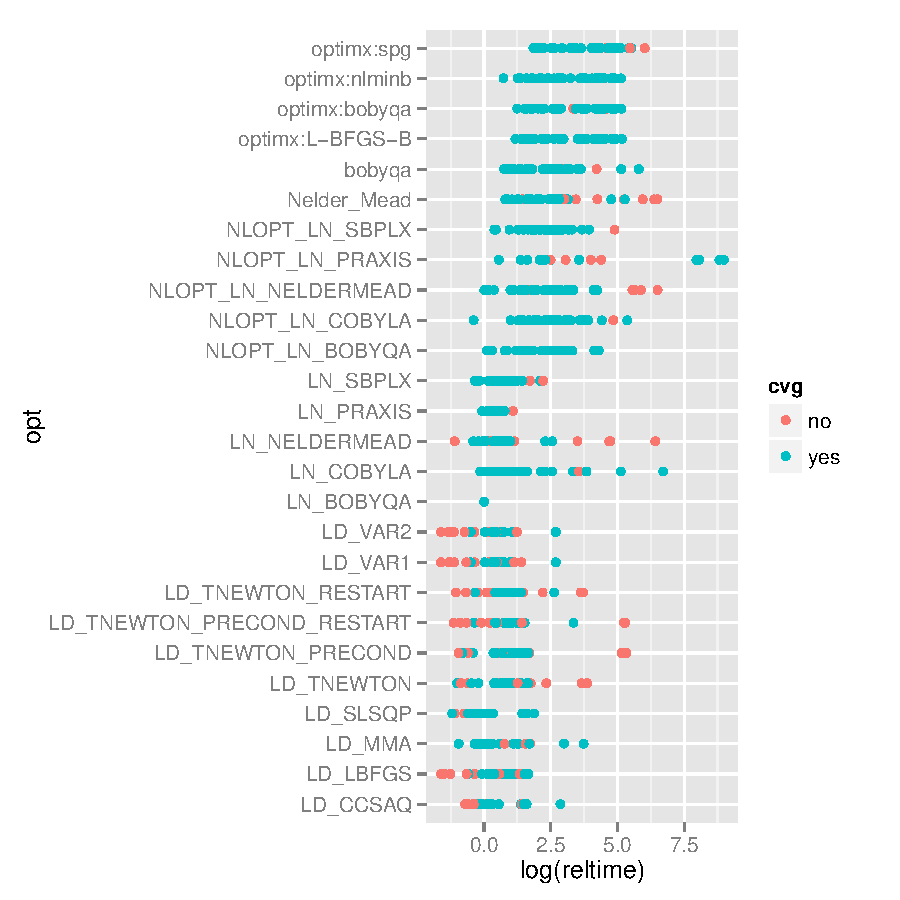
\includegraphics{Paper-013}


Many of the cases where LN_BOBYQA is slower than other algorithms are simple problems that converge in less than 1/5 of a second for most algorithms.

We will declare a data set to be non-simple if at least one of the models fit to the data took more than 0.2 seconds to convergence with LN_BOBYQA.

\begin{Schunk}
\begin{Sinput}
> print(xtable(subset(res, opt=="LN_BOBYQA" & time >= 0.2)[c("dsname","time","n","np","models")]),floating=FALSE, table.placement="H")
\end{Sinput}
% latex table generated in R 3.1.3 by xtable 1.7-4 package
% Thu Sep 24 15:26:31 2015
\begin{tabular}{rlrrrl}
  \hline
 & dsname & time & n & np & models \\ 
  \hline
354 & bs10 & 0.25 & 1104 &  20 & Y \~{} 1 + U + V + W + ((1 + U + V + W) $|$ G) + ((1 + U + V + W) $|$ H) \\ 
  360 & d3 & 106.94 & 130418 &   9 & Y \~{} 1 + U + ((1 + U) $|$ G) + ((1 + U) $|$ H) + ((1 + U) $|$ I) \\ 
  362 & dialectNL & 1.75 & 225866 &   6 & Y \~{} 1 + A + U + V + W + X + Z + T + (1 $|$ G) + ((0 + V + W + X) $|$ G) + ((1 + A + Z) $|$ H) + (1 $|$ I) \\ 
  370 & gb12 & 0.20 & 512 &  20 & Y \~{} 1 + S + T + U + V + W + X + Z + ((1 + S + U + W) $|$ G) + ((1 + S + T + V) $|$ H) \\ 
  376 & InstEval & 2.35 & 73421 &   2 & Y \~{} 1 + I * A + (1 $|$ G) + (1 $|$ H) \\ 
  377 & InstEval & 4.36 & 73421 &   3 & Y \~{} 1 + A + (1 $|$ G) + (1 $|$ H) + (1 $|$ I) \\ 
  378 & kb07 & 4.24 & 1790 &  72 & Y \~{} 1 + S + T + U + V + W + X + Z + ((1 + S + T + U + V + W + X + Z) $|$ G) + ((1 + S + T + U + V + W + X + Z) $|$ H) \\ 
  379 & kb07 & 0.70 & 1790 &  16 & Y \~{} 1 + S + T + U + V + W + X + Z + (1 $|$ G) + ((0 + S) $|$ G) + ((0 + T) $|$ G) + ((0 + U) $|$ G) + ((0 + V) $|$ G) + ((0 + W) $|$ G) + ((0 + X) $|$ G) + ((0 + Z) $|$ G) + (1 $|$ H) + ((0 + S) $|$ H) + ((0 + T) $|$ H) + ((0 + U) $|$ H) + ((0 + V) $|$ H) + ((0 + W) $|$ H) + ((0 + X) $|$ H) + ((0 + Z) $|$ H) \\ 
  381 & mm0 & 1.10 & 69588 &   6 & Y \~{} 1 + A * U + ((1 + U) $|$ G) + ((1 + U) $|$ H) \\ 
  386 & Poems & 5.69 & 275996 &   3 & Y \~{} 1 + U + V + (1 $|$ G) + (1 $|$ H) + (1 $|$ I) \\ 
   \hline
\end{tabular}\end{Schunk}



\subsection[Reliablility]{Reliability}

 Sed iaculis sodales elit quis vehicula. In et tristique neque, sodales aliquet metus. In posuere dictum nisl, quis laoreet augue congue a. Aenean in commodo neque, sit amet hendrerit ex. Aliquam id faucibus ante. Vivamus in fermentum nunc. Nam condimentum eros id orci pretium, quis aliquam magna eleifend. 

\section[Conclusions]{Conclusions}

\section[References]{References}



Douglas Bates, Katharine M. Mullen, John C. Nash and Ravi Varadhan (2014). minqa:
  Derivative-free optimization algorithms by quadratic approximation. R package version 1.2.4.
  http://CRAN.R-project.org/package=minqa

Bates D, Maechler M, Bolker B and Walker S (2014). _lme4: Linear mixed-effects models using Eigen
  and S4_. R package version 1.1-7, <URL: http://CRAN.R-project.org/package=lme4>.

John C. Nash, Ravi Varadhan (2011). Unifying Optimization Algorithms to Aid Software System
  Users: optimx for R. Journal of Statistical Software, 43(9), 1-14. URL
  http://www.jstatsoft.org/v43/i09/.

Jeroen Ooms (2014). The jsonlite Package: A Practical and Consistent Mapping Between JSON Data
  and R Objects. arXiv:1403.2805 [stat.CO] URL http://arxiv.org/abs/1403.2805.

Steven G. Johnson, The NLopt nonlinear-optimization package, http://ab-initio.mit.edu/nlopt
  
(For the nloptr package they want us to go through and cite each algorithm we used)  
  
\end{document}
